\documentclass[a4paper,14pt]{article}
\usepackage{float}
\usepackage{extsizes}
\usepackage{amsmath}
\usepackage{amssymb}
\everymath{\displaystyle}
\usepackage{geometry}
\usepackage{fancyhdr}
\usepackage{multicol}
\usepackage{graphicx}
\usepackage[brazil]{babel}
\usepackage[shortlabels]{enumitem}
\usepackage{cancel}
\usepackage{textcomp}
\usepackage{array} % Para melhor formatação de tabelas
\usepackage{longtable}
\usepackage{booktabs}  % Para linhas horizontais mais bonitas
\usepackage{float}   % Para usar o modificador [H]
\usepackage{caption} % Para usar legendas em tabelas
\usepackage{tcolorbox}
\usepackage{wrapfig} % Para usar tabelas e figuras flutuantes

\columnsep=2cm
\hoffset=0cm
\textwidth=8cm
\setlength{\columnseprule}{.1pt}
\setlength{\columnsep}{2cm}
\renewcommand{\headrulewidth}{0pt}
\geometry{top=1in, bottom=1in, left=0.7in, right=0.5in}

\pagestyle{fancy}
\fancyhf{}
\fancyfoot[C]{\thepage}

\begin{document}
	
	\noindent\textbf{6FMA58 - Matemática} 
	
	\begin{center}Operações com potências de 10 (Versão estudante)
	\end{center}
	
	\noindent\textbf{Nome:} \underline{\hspace{10cm}}
	\noindent\textbf{Data:} \underline{\hspace{4cm}}
	
	%\section*{Questões de Matemática}
	\begin{multicols}{2}
    		\noindent 
    		\begin{itemize}
    			\item Para multiplicarmos um número decimal por 10, 100, 1000, ..., deslocamos a vírgula, respectivamente, 1, 2, 3, ... casas para a direita e a partir da posição inicial.
    			\item Para dividirmos um número decimal por 10, 100, 1000, ..., deslocamos a vírgula, respectivamente, 1, 2, 3, ... casas para a esquerda a partir da posição inicial.
    		\end{itemize}
    		\noindent Exemplos:
    		\begin{itemize}
    			\item $1,257 \cdot 100 = 125,7$
    			\item $9,87 \cdot 10000 = 98700$
    			\item $37,5 : 10 = 3,75$
    			\item $0,02 : 1000 = 0,00002$
    		\end{itemize}
    		\textsubscript{---------------------------------------------------------------------}
    		\begin{enumerate}
    			\item Escreva como decimal:
    			\begin{enumerate}[a)]
    				\item $\frac{36}{100}$ \\\\\\
    				\item $865 : 100$ \\\\\\
    				\item $1974 : 10000$ \\\\\\
    				\item 18 dividido por 1000 \\\\\\
    				\item o quociente de 721 por 100 \\\\\\
    			\end{enumerate}
    			\item Calcule:
    			\begin{enumerate}[a)]
    				\item $1,72 \cdot 10$ \\\\\\
    				\item $1,72 : 10$ \\\\\\
    				\item $30,6 \cdot 10$ \\\\\\
    				\item $30,6 : 10$ \\\\\\
    				\item $1,39 \cdot 100$ \\\\\\
    				\item $1,39 : 100$ \\\\\\
    				\item $64,128 \cdot 1000$ \\\\\\
    				\item $64,128 : 1000$ \\\\\\
    				\item $1,3074 \cdot 1000$ \\\\\\
    				\item $1,3074 : 1000$ \\\\\\
    			\end{enumerate}
    			\item Complete o diagrama: \\
    			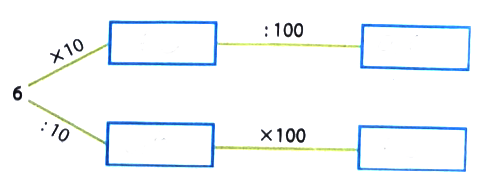
\includegraphics[width=1.1\linewidth]{6FMA58_imagens/imagem1} \\\\
    			\textbf{Desafio olímpico} \\\\
    			Das alternativas abaixo, a mais próxima de 25,07 $\times$ 400,21 é: \\
    			\begin{enumerate}[a)]
    				\item 1 000
    				\item 10 000
    				\item 100 000
    				\item 1 000 000
    				\item 100 000 000
    			\end{enumerate}
    			% 29 a 32
    			\item Escreva como decimal:
    			\begin{enumerate}[a)]
    				\item $\frac{19}{100}$ \\\\\\
    				\item $392 : 100$ \\\\\\
    				\item $4 803 : 10 000$ \\\\\\
    				\item 92 dividido por 1 000 \\\\\\
    				\item o quociente de 288 por 100 \\\\\\
    			\end{enumerate}
    			\item Calcule:
    			\begin{enumerate}[a)]
    				\item $15,2 \cdot 10$ \\\\\\
    				\item $15,2 : 10$ \\\\\\
    				\item $7,21 \cdot 10$ \\\\\\
    				\item $7,21 : 10$ \\
    				\item $0,946 \cdot 100$ \\\\\\
    				\item $0,946 : 10$ \\\\\\
    				\item $11,426 \cdot 1 000$ \\\\\\
    				\item $11,426 : 1 000$ \\\\\\
    			\end{enumerate}
    			\item O número 1 234 567 890 representa quantas vezes o número 0,0123456789? \\\\\\
    			\item Multiplicamos um número decimal por 10 e, em seguida, dividimos o resultado por 10 000. Multiplicamos o número obtido por $10^8$ e dividimos o resultado por 1 bilhão. Qual é a posição da vírgula em relação à posição inicial?
    		\end{enumerate}
    		$~$ \\ $~$ \\ $~$ \\ $~$ \\ $~$ \\ $~$ \\ $~$ \\ $~$ \\ $~$ \\ $~$ \\ $~$ \\ $~$ \\ $~$ \\ $~$ \\ $~$ \\ $~$ \\ $~$ \\ $~$ \\ $~$ \\ $~$ \\ $~$ \\ $~$ \\ $~$ \\ $~$ \\ $~$ \\ $~$ \\ $~$ \\ $~$ \\ $~$ \\ $~$ \\ $~$ \\ $~$ \\ $~$ \\ $~$ \\ $~$ \\ $~$ \\ $~$ \\ $~$ \\ $~$ \\ $~$ \\ $~$ \\ $~$ \\ $~$ \\ $~$ \\ $~$ \\ $~$ \\ $~$ \\ $~$ \\ $~$
	\end{multicols}
\end{document}